% Para iniciar una sección debe escribirse
%\section{Nombre de la sección}
% Lo anterior inmediatamente creará la sección y la numerará.

\section*{Objetivos}
\subsection*{Generales}
\begin{itemize}
    \item Diseñar y construir un circuito secuencial capaz de generar señales analógicas.
\end{itemize}

\subsection*{Específicos}
\begin{itemize}
    \item Diseñar múltiples circuitos secuenciales para obtener un resultado único en conjunto
    \item Generar una señal digital de modulación de ancho de pulso (PWM)
    \item Implementar un circuito de lógica secuencial capaz de establecer la rapidez de un motor a través de PWM
    \item Contrastar los diseños teóricos con los resultados experimentales de los circuitos implementados físicamente
\end{itemize}

% \section{Introducción}

% \subsection{Aritmética binaria}
% Los dispositivos digitales se basan en operaciones con numeración \emph{base 2} para obtener los resultados, incluso si la interfaz de usuario tuviese otro 
% formato (numérico decimal, en base a gráficos o imágenes, etc.). Las operaciones aritméticas en \emph{base 2} cumplen con los mismos teoremas y reglas que se
% utilizan en base 10, pero poseen la ventaja de tener más simplificaciones debido a la limitada cantidad de dígitos disponibles. Consulte su libro de
% texto\footnote{Mano, Morris. Digital Design, 5th edition} para recapitular lo anteriormente descrito.

% \pagebreak

\section{Desarrollo Experimental}
\subsection{Materiales y Equipo}

Cada grupo debe llevar su material y equipo de trabajo durante las prácticas. Pregunte a su profesor qué \emph{Equipo de Laboratorio} puede ser prestado
de parte del laboratorio de instrumentación. El laboratorio de instrumentación no tiene disponibilidad de ningún elemento de la lista \emph{Materiales}.

\subsubsection*{Materiales}
\begin{itemize}
    \item 1x fuente de alimentación (ver apartado anterior con todas las alternativas)
    \item 2x capacitores electrolíticos de 47 $\mu$F 16V
    \item 2x capacitores cerámicos de 100nF 25V
    \item 5x resistencias de 1 k$\ohm$ para pull-down/pull-up
    \item 1x resistencia de 10 k$\ohm$ para compuerta de MOSFET
    \item 1x LED de cualquier color
    \item 1x pulsador como reset del sistema
    \item 1x Resistencia $220 \ohm \leq R \leq 1 k\ohm$
    \item 1x circuito integrado temporizador 555
    \item 2x Resistencias para temporización de reloj
    \item 1x Capacitor para temporización de reloj
    \item 1x Capacitor $10nF \leq C \leq 100nF$
    \item 1x Motor de 3VDC o 5VDC (puede ser reciclado de un juguete que no estén utilizando)
    \item 1x MOSFET voltaje de umbral lógico, canal tipo N. Si la corriente del motor no supera 200 mA, puede utilizar un 2N7000. De lo contrario, consulte a su instructor
            de laboratorio.
    \item 1x diodo de silicio de 1A, al menos de 25V (puede ser 1N4001, 1N4002, ... , 1N4007)
    \item Flip-flops de acuerdo a su diseño (si se requiere usar tipo \emph{T}, puede adquirir FFs tipo \emph{JK})
    \item Las compuertas lógicas a utilizar dependen del diseño final de cada grupo (AND, OR, NOT, XOR, NAND, XNOR)
    \item 6x metros de alambre para protoboard calibre 22. Compren al menos 2 colores para los 6 metros. \textbf{No usen \emph{UTP}}, aunque eso les quieran vender.
\end{itemize}


\subsubsection*{Equipo de Laboratorio}
\begin{itemize}
    \item 1x Pinzas delgadas
    \item 1x Cortaalambres
    \item 1x Pelador de alambres para calibre 22 (opcional)
    \item 1x Tijeras pequeñas o cortauñas (si no tienen pela alambres)
    \item 1x Protoboard de al menos 2 galletas (puede juntar 2 protoboards de 1 galleta)
    \item 1x Multímetro digital para medir voltaje
\end{itemize}

\subsection{Procedimiento}
\subsubsection{Fuente de alimentación}
Utilice la misma fuente de alimentación que en la Práctica \#1.

\subsection{Reloj del sistema}
Diseñe un reloj de frecuencia constante y ciclo de trabajo cercano al 50\% para controlar la lógica combinacional del proyecto. Utilice un temporizador 555 haciendo uso de las 
ecuaciones de diseño en modo astable. Tome en cuenta que para el diseño del sistema cada ciclo de reloj puede significar un aumento de valor en la lógica, por lo que el período de cada pulso.

Es imprescindible que la frecuencia de operación de PWM sea calculada para funcionar correctamente con los parámetros del motor que utilizará, la cuál a su vez, 
depende de la frecuencia de reloj del sistema.

\subsubsection{PWM}
Utilizando los conocimientos adquiridos en las prácticas de laboratorio anterior y la teoría de contadores y registros debe implementar un sistema que 
genere una señal de frecuencia constante con variación de ancho de pulso (PWM). El objetivo es generar un modulador de N = 4 bits.

El usuario debe establecer el ciclo de trabajo deseado entre $0 \leq D \leq 2^{N}-1$ utilizando un dip-switch.

El resultado debe ser una salida digital PWM de 1 bit con la frecuencia (constante) adecuada para manejar el motor.

Es requisito entrega la memoria de cálculo de la frecuencia mínima de la señal de reloj y de la señal de PWM para tener derecho a la entrega de la práctica de laboratorio.

\subsection{Amplificador de potencia}
Para controlar un dispostivo que consuma mucha corriente para su funcionamiento (e.g. el motor o una bocina) no se posible conectar directamente la 
señal digital hacia el transductor, de lo contrario la potencia entregada por la compuerta/FF estaría muy por encima de las especificaciones del fabricante,
dañando permanentemente el circuito integrado (y posiblemente el resto del circuito).

El amplificador de potencia obteiene una señal que proviene de un dispositivo de baja potencia y entrega dicha señal (prácticamente sin distorsión) al transductor
o dispositivo que requiera una potencia mayor para funcionar, esto sin dañar la lógica digital que se encuentre detrás.

Para un motor la configuración más simple es utilizar un transistor MOSFET en modos de corte/saturación para replicar un estado lógico (0/1 respectivamente). 
En la Figura \ref{Fig:MOSFETDRIVER} se muestra el esquema de conexión simple para conectar el motor al sistema digital. Note que si el motor consume una potencia mayor a 
3/4 de Watt en el estado estable y sin carga, deberá colocar un diodo de protección entre VDD y el drejane del MOSFET.


\begin{figure}[H]
    \centering
    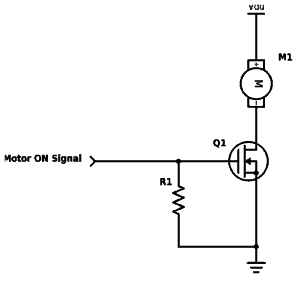
\includegraphics[scale=0.8]{images/motorMOSFET.png}
    \caption{Esquema de conexión para amplificador de potencia}
    \label{Fig:MOSFETDRIVER}
\end{figure}

\subsection{Interfaz de usuario}
El usuario deberá establecer en codificación binaria el valor de PWM que desea a la salida utilizando los 4 dip-siwtch. La salida será simplemente
el motor conectado al amplificador de potencia. Se recomienda utilizar un LED (con resistencia en serie) para realizar las pruebas antes de conectar 
el circuito de amplificación de potencia.  El eje del motor debe tener conectado algún distintivo (masking-tape, por ejemplo) que permita verificar 
cuando se ha realizado una revolución.

Al momento de calificar se utilizará un osciloscopio para verificar la señal generada por el circuito; asimismo, se utilizará una cámara de alta velocidad
para determinar que los cambios de ciclo de trabajo afecten realmente a la rapidez de rotación del motor.

\section{Recomendaciones}
Para realizar las pruebas de funcionamiento sin la necesidad de utilizar equipo sofisticado de medición (osciloscopio), puede cambiar el capacitor del reloj del sistema
de tal forma que la señal de reloj disminuya a una frecuencia distinguible fácilmente por el ojo humano (dígase 1 Hz). Note que la frecuencia a la que originalmente
debe trabajar el sistema para que la señal PWM funcione adecuadamente con el motor debe estar muy por encima de 2 kHZ.